% v2-acmtog-sample.tex, dated March 7 2012
% This is a sample file for ACM Transactions on Graphics
%
% Compilation using 'acmtog.cls' - version 1.2 (March 2012), Aptara Inc.
% (c) 2010 Association for Computing Machinery (ACM)
%
% Questions/Suggestions/Feedback should be addressed to => "acmtexsupport@aptaracorp.com".
% Users can also go through the FAQs available on the journal's submission webpage.
%
% Steps to compile: latex, bibtex, latex latex
%
% For tracking purposes => this is v1.2 - March 2012
\documentclass{sig-alternate} % V1.2

%\acmVolume{VV}
%\acmNumber{N}
%\acmYear{YYYY}
%\acmMonth{Month}
%\acmArticleNum{XXX}
%\acmdoi{10.1145/XXXXXXX.YYYYYYY}
\usepackage{graphicx}
%\usepackage[T2A]{fontenc} 
%\usepackage[utf8]{inputenc}
\usepackage{graphicx}
%\usepackage{indentfirst}
\usepackage{hyperref}
\usepackage{textcomp}

\begin{document}

\makeatletter
\def\@copyrightspace{\relax}
\makeatother

\title{Generalized LL parsing for context-free constrained path search problem}

\sloppy

\numberofauthors{2}

\author{
\alignauthor
       Semyon Grigorev\\
       \affaddr{Saint Petersburg State University}\\
       \affaddr{7/9 Universitetskaya nab.}\\
       \affaddr{St. Petersburg, 199034 Russia}\\
       \email{rsdpisuy@gmail.com}
\alignauthor
       Anastasiya Ragozina\\
       \affaddr{Saint Petersburg State University}\\
       \affaddr{7/9 Universitetskaya nab.}\\
       \affaddr{St. Petersburg, 199034 Russia}\\
       \email{ragozina.anastasiya@gmail.com}
}

\maketitle

\begin{abstract}
Aaaabstract

\end{abstract}

\section{Introduction}
Graph data model and graph data bases are very popular in many different areas such as bioinformatic, semantic web, social networks etc.
Extraction of paths satisfying specific constraints may be useful for graph structured data investigation and for relations between data items detection.
Path querying with constrains formulated in terms of formal grammars is a specific problem named formal language constrained path problem~\cite{FLCpathProblem} and research in this area is still actual~\cite{DirOfBigGraphAnalysis}.

\section{Releted work}

relaxed rnglr~\cite{relaxedRNGLR}

\section{Preliminaries}

Let we introduce some definitions.
\begin{itemize}
  \item Context-free grammar $G=(N, \Sigma, P, S)$ where $N$ is a set of nonterminal symbols, $\Sigma$ is a set of nonterminal symbols, $S \in N$ is a start nionterminal, and $P$ is a productions set. 
  \item Directed graph $M = (V,E,L)$ where $V$ --- vertices set, $L \subseteq \Sigma$ --- edge labels set, $E\subseteq V\times L\times V$.
  \item Helper function $tag: E \rightarrow L; tag(e = (v_1,l,v_2), e \in E) = l$.
  \item Concatenation operation $\oplus: L^+ \times L^+ \rightarrow L^+$.
  \item Path $p$ in graph $M$. \\ $p = (v_0,l_0,v_1),(v_1,l_1,v_2),\dots,(v_{n-1},l_{n-1},v_n) = e_0,e_1,\dots,e_{n-1}$ where $v_i \in V$,$e_i \in E$, $l_i \in L$, $|p| = n \leq 1$. 
  \item Set of path $P = \{p: p \text{ path in } M\}$
  \item Helper function $\Omega: P \rightarrow L^+$.\\ $\Omega(p = e_0,e_1,\dots,e_{n-1}, p \in P) = tag (e_0) \oplus \dots \oplus tag (e_{n-1})$.
\end{itemize}

As a result we can define that context-free language constrained path querying meens that each path $p = e_0,\dots,e_{n-1}$ from result set satisfied with next constraint: $\Omega(p) \in L(G)$. 

As a motivation of context-free constraints importance let we introduce the next example.
Let we have graph $M=(\{0;1;2;3\},E,\{A;B\})$ presented in figure~\ref{input} where labels represent $parent (A)$ and $child (B)$ relations. 
Suppose for each $n \leq 1$ we want to find all $n$-th generation descendants with a common ancestor.
In the other worlds, we wath to find all paths $p$, such that $\Omega(p) \in \{AB; AABB; AAABBB; \dots\}$ or $\Omega(p) = A^n B^n$ where $n \geq 1$.
This constraint can not be specified with regular language as far as $L=\{A^n B^n; n \geq 1\}$ is not regular but context free.
Required language can be specified by grammar $G$ presented in picture~\ref{grammarG} where $N = \{s; middle\}$, $\Sigma = \{A; B\}$, and $S = s$.

\begin{figure}[h]
    \begin{center}
        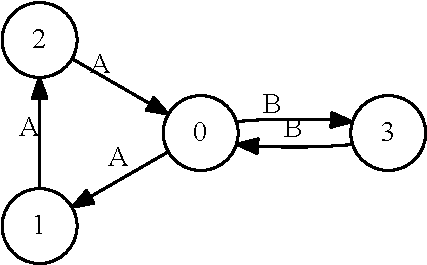
\includegraphics[width=6cm]{dot/input.pdf}
        \caption{Input graph $M$}
        \label{input}        
    \end{center}
\end{figure}

\begin{figure}[h]
   \begin{center}
\begin{verbatim}
s: A s B | middle
middle: A B
\end{verbatim}
   \caption{Grammar $G$ for language $L=\{A^n B^n; n \geq 1\}$}
   \label{grammarG}        
   \end{center}
\end{figure}

\section{Proposed algorithm}
We propose a context-free language constrained path problem solution which allow to find all paths satisfied specified arbitrary context-free grammar and to construct implicit representation of result. 
Finite representation of result set with structure related to specified grammar may be useful not only for results understanding and processing but also for query debugging especially for complex queries. 

Our solution is based on generalized LL (GLL)~\cite{scott2010gll, FastPracticalGLL} parsing algorithm which allow to process ambiguous context-free grammars.
Complexity is $O(n^3)$ in worst case and linear for unambiguous grammars, that better then complexity of CYK and Earley which used as base in other solutions (for example~\cite{ConjCFPathQuery}, ~\cite{GraphQueryWithEarley}).
This fact allow to demonstarte better performance on linear subgraphs and unambiguous grammars.
Also it is not necessary to transform input grammar to CNF which required for CYK.

\section{Example}
In details, main function input is graph $M$, set of start vertices $V_s\subseteq V$, set of final vertices $V_f\subseteq V$, grammar $G$.
Output is Shared Packed Parse Forest (SPPF)~\cite{SPPF} --- finite data structure which contains all derivation trees for all paths in $M$, $\Omega(p) \in L(G)$ and allows to reconstruct any of paths implicitly.
As far as we can specify sets of start and final vertices, our solution can find all paths in graph, all paths from specified vertex, all paths between specified vertices. 
Also SPPF represents a structure of paths in terms of derivation which allow to get more useful information about result.

Let we introduce the next example. Grammar $G$ is a query and we want to find all paths in graph $M$ (presented in picture~\ref{input}) matched this query.
Result SPPF for this input is presented in picture~\ref{SPPF}. 

\begin{figure}[h]
    \begin{center}
        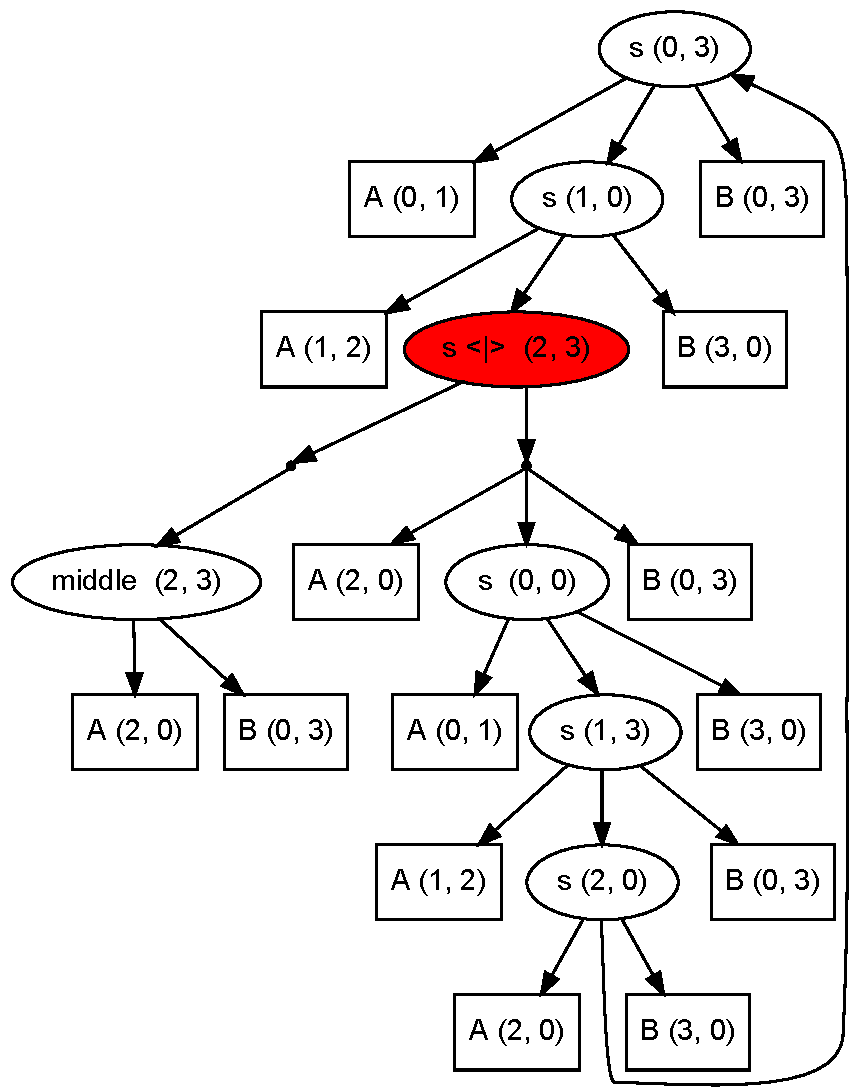
\includegraphics[width=9cm]{dot/AnBn.pdf}
        \caption{Result SPPF for input graph $M$(pic.~\ref{input}) and query $G$(pic.~\ref{grammarG})}
        \label{SPPF}        
    \end{center}
\end{figure}

We use next markers for nodes.
\begin{itemize}
    \item Node with rectangle shape labeled with $(v_0, T, v_1)$ is terminal node. 
    Each terminal node corresponds with edge in the input graph: for each node with label $(v_0, T, v_1)$ there is $e\in E: e=(v_0,T,v_1)$.
    Duplication of terminal nodes is only for figure simplification.
    \item Node with oval shape labeled with $(v_0, nt, v_1)$ is nonterminal node. 
    This node denote that there is at least one path $p$ from vertex $v_0$ to vertex $v_1$ in input graph $M$ such that $nt \Rightarrow^*_G \Omega(p)$.
    All paths matched this condition can be extracted from SPPF by left-to-right top-down graph traversal started from respective node. 
    \item Filled node with oval shape labeled with $(<\mkern-11mu | \mkern-11mu> (v_0, nt, v_1))$ is nonterminal node denote that there are more then one path from $v_0$ to $v_1$ such that $nt \Rightarrow^*_G \Omega(p)$.
    \item Node with dot shape is used for representation of derivation variants.
    Subgraph with root in one such node is one variant of derivation.
    Parent of such nodes is always node with label $(<\mkern-9mu | \mkern-9mu> (v_0, nt, v_1))$.
    \item $v_0$ and $v_1$ are left and right extensions of node respectively.
\end{itemize}

As an example of derivation structure usage we can find 'middle' of any path in example above simply by finding corresponded nonterminal $middle$ in SPPF.
So we can found that there is only one common ancestor for all results and it is vertex with id=$0$. 

Extensions stored in nodes allow to check whether path from $u$ to $v$ exists and extract it. 
Path extraction is SPPF traversal. 
Let for example we want to find path satisfying specified constraints fron vertex $0$.
To do this we should find vertices with label $(0, s, \_)$ in SPPF. There are two vertices: $(0, s, 0)$ and $(0, s , 3)$.
In our example there is cycle in SPPF so there are \textbf{at least} two different paths: $p_0=\{(0,A,1);(1,A,2);(2,A,0);(0,B,3);(3,B,0);(0,B,3)\}$ and $p_1=\{(0,A,1);(1,A,2);(2,A,0);(0,A,1);(1,A,2);(2,A,0);\\ (0,B,3);(3,B,0);(0,B,3);(3,B,0);(0,B,3);(3,B,0)\}$ .

\section{Evaluation}

\section{Conclusion and future work}
We propose GLL-based algorithm for context-free path querying which construct finite structural representation of all paths satisfying given constrains.
Provided data structure can be useful for result investigation and processing, and debugging.
Presented algorithm implemented in F\# and available on GitHub:\url{https://github.com/YaccConstructor/YaccConstructor}.

Our future work is theoretical complexity estimation.
Improve performance~\cite{FGLL}


\bibliographystyle{abbrv}
\bibliography{ContextFreeConstrainedPathFindingInGraph}

%\bibitem{PathQuerySemantic}
%Hellings, J. (2015). Querying for Paths in Graphs using Context-Free Path Queries. arXiv preprint 
%arXiv:1502.02242.

%\bibitem{CFPathQuery}
%Sevon, P., /& Eronen, L. (2008). Subgraph queries by context-free grammars. Journal of Integrative 
%Bioinformatics, 5(2), 100.


\end{document}
